% Provenance (never printed): old terminale S material on the early Earth (the
% primitive atmosphere and its outgassing, the first traces of life, the rise of
% oxygen read in the rocks: banded iron formations, red beds) and the faint young
% Sun. Owner (Sync 0/1): outgassing and primitive atmosphere, faint young Sun
% problem, stromatolite, Great Oxidation Event, banded iron formation, red beds.
% Recalled: age of the Earth (g12.07), zircons (g12.01), equilibrium temperature
% (g10.02), photosynthesis and cyanobacteria (biology), air composition, greenhouse
% gases as molecules and redox (chemistry). Figures: figdata/grade-12/early_earth.py.
\chapter{La Terre primitive et son atmosphère}\label{ch:g12:early-earth}

Dans les monts Hamersley, au nord-ouest de l'Australie, les parois de Dales
Gorge sont rayées comme un gâteau à étages~: de fines bandes de roche rouge,
grise et noire. C'est une \omterm{def:g12:early-earth:bif}{formation de fer rubané}, déposée sur un fond
marin il y a plus de 2.5~milliards d'années. Le fer qu'elle contient a
rouillé dans cette mer, et pour rouiller, il lui fallait de l'oxygène. Ce
chapitre cherche à quoi ressemblaient la jeune Terre et son air, et comment
les roches enregistrent le moment où l'oxygène est apparu.
% ledger: dbca:karijini, earle:bif, photo:g12-dales-gorge

\begin{omfigure}
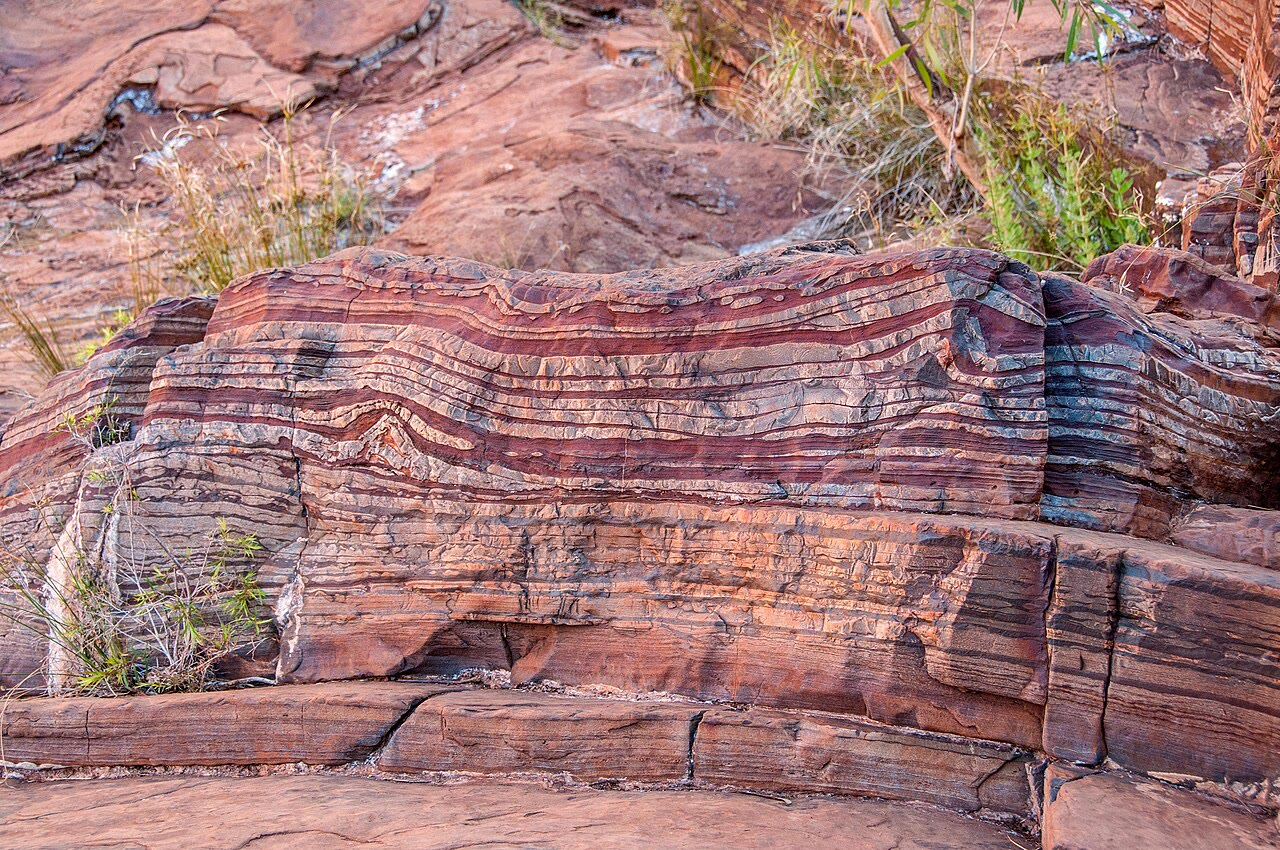
\includegraphics[width=0.72\linewidth]{images/book2/g12-dales-gorge-bif.jpg}

{\small \omterm{def:g12:early-earth:bif}{Formation de fer rubané} aux chutes Fortescue, Dales Gorge, parc
national de Karijini, Australie-Occidentale. Photographie Graeme Churchard,
CC~BY~2.0 (Wikimedia Commons).}
\end{omfigure}

\begin{recall}
La Terre a 4.54~milliards d'années (\cref{ch:g12:age-of-the-earth}), et
des zircons montrent qu'une croûte existait il y a 4.4~milliards d'années
(\cref{ch:g12:continental-crust}). La \omterm{def:g10:habitable-planet:equilibrium-temperature}{température d'équilibre} d'une planète,
$T_{\mathrm{eq}} = \left(S(1-A)/(4\sigma)\right)^{1/4}$, vaut environ
\qty{255}{K} pour la Terre actuelle (\cref{ch:g10:habitable-planet}).
L'air sec actuel contient \qty{78}{\percent} d'azote et \qty{21}{\percent}
d'oxygène, et le dioxyde de carbone et le méthane sont des gaz à effet de
serre~; un élément qui fixe de l'oxygène est oxydé (les livres de chimie).
Les plantes, les algues et les cyanobactéries fabriquent leur nourriture
par photosynthèse, qui libère de l'oxygène (les livres de biologie).
\end{recall}
% ledger: usgs:age-earth (Book 1 row), wilde01:zircon, earth:TSI, earth:albedo, air:N2, air:O2

\section{La jeune Terre}

La Terre a grossi par accrétion de corps plus petits. Environ 60 millions
d'années après le début de la formation du système solaire, un corps de la
taille de Mars peut-être la heurta, et la matière projetée dans l'espace
forma la Lune. La jeune Terre était chaude et encore en partie fondue. Elle
se refroidit, et dès il y a environ 4.4~milliards d'années elle possédait
déjà une croûte et un océan~: des zircons de cet âge portent la marque
chimique de l'eau liquide.
% ledger: nasa:moon-formation, wilde01:zircon

\section{L'atmosphère primitive}

\begin{definition}[Dégazage~; atmosphère primitive]\label{def:g12:early-earth:primitive-atmosphere}
Le \emph{dégazage}\index{degazage@dégazage} est la libération, par les
volcans et à travers le sol, des gaz dissous dans le magma.
L'\emph{atmosphère primitive}\index{atmosphere primitive@atmosphère primitive}
est l'atmosphère de la Terre avant que les êtres vivants ne la modifient~:
formée surtout par dégazage, elle contenait de l'azote, du dioxyde de
carbone et de la vapeur d'eau, davantage de dioxyde de carbone
qu'aujourd'hui, et presque pas d'oxygène libre.
\end{definition}
% ledger: usgs:volcanic-gases (Book 1 row), holland06:stages (stage 1 anoxic), feulner12:fys (more carbon dioxide)

Les volcans montrent encore comment se forme une telle atmosphère~: à
mesure que le magma monte et que la pression baisse, ses gaz dissous
s'échappent, de loin le plus abondant étant la vapeur d'eau, puis le dioxyde
de carbone. L'azote et le dioxyde de carbone, les gaz qui dominaient l'air
primitif, sont encore aujourd'hui les principaux gaz azotés et carbonés des
volcans. La vapeur d'eau se condensa en océan. L'oxygène représentait moins
de \qty{0.001}{\percent} de sa teneur dans l'air actuel.
% ledger: usgs:volcanic-gases (Book 1 row), pk02:anoxic

Le jeune Soleil brillait moins qu'aujourd'hui. À mesure qu'il transforme
l'hydrogène en hélium dans son cœur, ce cœur se contracte et s'échauffe, et
la puissance du Soleil augmente lentement.

\begin{proposition}[La luminosité du jeune Soleil]\label{prop:g12:early-earth:luminosity}
En notant $t_\odot$ l'âge actuel du Soleil et $L_\odot$ sa luminosité
actuelle, sa luminosité quand il avait $t$ années valait
\[
  L(t) = \frac{L_\odot}{1 + \frac{2}{5}\left(1 - t/t_\odot\right)} .
\]
\end{proposition}
% ledger: gough81:luminosity, connelly12:cai

Cette approximation des modèles calculés du Soleil est admise ici. À la
naissance du Soleil, $t = 0$, elle donne $L = L_\odot/1.4 \approx 0.71\,L_\odot$~:
le jeune Soleil était environ \qty{30}{\percent} moins lumineux.

\begin{example}[La Terre il y a quatre milliards d'années]\label{ex:g12:early-earth:young-sun}
Prenons $t_\odot = 4.567$~milliards d'années. Il y a quatre milliards
d'années, le Soleil avait 0.567~milliard d'années~; donc
$1 - t/t_\odot = 4/4.567 \approx 0.876$ et
$L \approx L_\odot/1.350 \approx 0.741\,L_\odot$. La lumière solaire qui
atteignait la Terre valait $0.741 \times 1361 \approx \qty{1008}{W/m^2}$.
En gardant l'\omterm{def:g10:earth-energy-budget:albedo}{albédo} actuel, la \omterm{def:g10:habitable-planet:equilibrium-temperature}{température d'équilibre} varie comme la
racine quatrième de la lumière solaire~: $255 \times 0.741^{1/4} \approx 255 \times 0.928 \approx
\qty{237}{K}$, soit environ \qty{-36}{\celsius}.
\end{example}
% values: L_4Ga 0.7406, S_4Ga 1007.9, Teq_today 255.1, Teq_4Ga 236.7 (early_earth.py)

\begin{omfigure}
\begin{tikzpicture}
\begin{axis}[omrecord, scale only axis, width=0.66\linewidth, height=4.6cm,
  xmin=0, xmax=4.6, ymin=225, ymax=295, x dir=reverse, axis y line*=left,
  xlabel={temps avant l'actuel (milliards d'années)}, ylabel={température (K)},
  xtick={0,0.5,...,4.5}, x tick label style={/pgf/number format/.cd, fixed, precision=1}]
% computed in figdata/grade-12/early_earth.py; ledger: gough81:luminosity, earth:TSI, earth:albedo, earth:Tsurf
\addplot[omDef, line width=1.2pt] table[x=t_Ga, y=Teq] {figdata/out/grade-12-early_earth-sun.dat};
\addplot[omThm, densely dashed, domain=0:4.6, samples=2] {273.15};
\addplot[black!60, densely dotted, domain=0:4.6, samples=2] {288};
\coordinate (teq) at (axis cs:2.6,239);
\coordinate (frz) at (axis cs:2.3,274);
\coordinate (sfc) at (axis cs:2.3,289);
\end{axis}
\begin{axis}[omrecord, scale only axis, width=0.66\linewidth, height=4.6cm,
  xmin=0, xmax=4.6, ymin=0.65, ymax=1.05, x dir=reverse, axis y line*=right, axis x line=none,
  ylabel={luminosité du Soleil ($L_\odot$)}, ymajorgrids=false, xmajorgrids=false,
  y tick label style={/pgf/number format/.cd, fixed, fixed zerofill, precision=2}]
\addplot[omProp, line width=0.9pt, densely dashdotted] table[x=t_Ga, y=L] {figdata/out/grade-12-early_earth-sun.dat};
\coordinate (lum) at (axis cs:1.7,0.86);
\end{axis}
\node[font=\scriptsize, text=omDef, anchor=north] at (teq) {température d'équilibre};
\node[font=\scriptsize, text=omThm, anchor=south] at (frz) {l'eau gèle, \qty{273}{K}};
\node[font=\scriptsize, text=black!70, anchor=south] at (sfc) {surface moyenne actuelle, \qty{288}{K}};
\node[font=\scriptsize, text=omProp, anchor=north west] at (lum) {luminosité (échelle de droite)};
\end{tikzpicture}

{\small Le jeune Soleil faible~: sa luminosité (échelle de droite) et la
\omterm{def:g10:habitable-planet:equilibrium-temperature}{température d'équilibre} de la Terre avec l'\omterm{def:g10:earth-energy-budget:albedo}{albédo} actuel (échelle de
gauche), jusqu'à la naissance du Soleil. Calculé d'après Gough (1981) avec
la lumière solaire et l'\omterm{def:g10:earth-energy-budget:albedo}{albédo} actuels.}
\end{omfigure}

\begin{definition}[Paradoxe du jeune Soleil faible]\label{def:g12:early-earth:faint-young-sun}
Le \emph{paradoxe du jeune Soleil faible}\index{paradoxe du jeune Soleil faible}
est la contradiction entre le Soleil moins lumineux des premiers milliards
d'années de la Terre, sous lequel la Terre, avec l'atmosphère actuelle,
aurait gelé, et les roches, qui montrent que de l'eau liquide était
présente.
\end{definition}
% ledger: feulner12:fys

Le problème fut largement connu en 1972 grâce à Carl Sagan et George
Mullen, qui proposèrent comme réponse un effet de serre plus fort. La
plupart des réponses étudiées depuis font appel à davantage de gaz à effet
de serre dans l'\omterm{def:g12:early-earth:primitive-atmosphere}{atmosphère primitive}~: beaucoup plus de dioxyde de carbone
qu'aujourd'hui, du méthane produit par les premiers microbes, ou les deux.
Selon un calcul classique, environ un dixième de bar de dioxyde de carbone,
avec un peu de méthane, maintient la jeune Terre aussi chaude
qu'aujourd'hui~; sans le méthane, il en faut environ trois fois plus. On ne
considère pas encore le problème comme résolu.
% ledger: feulner12:fys

\section{La vie et l'oxygène}

Les \omterm{def:g12:early-earth:stromatolite}{stromatolithes} fossiles couvrent près de \num{3500} millions
d'années~: ils comptent parmi les plus anciennes traces de vie.

\begin{definition}[Stromatolithe]\label{def:g12:early-earth:stromatolite}
Un \emph{stromatolithe}\index{stromatolithe} est un monticule lité
construit en eau peu profonde par un tapis de microbes, surtout des
cyanobactéries, qui piègent et lient des grains de sédiment et font croître
du carbonate, couche après couche.
\end{definition}
% ledger: noffke13:stromatolites

On trouve des \omterm{def:g12:early-earth:stromatolite}{stromatolithes} fossiles de \num{3430} millions d'années dans
le chert de Strelley Pool, dans le Pilbara, en Australie-Occidentale. Des
\omterm{def:g12:early-earth:stromatolite}{stromatolithes} vivants croissent aujourd'hui dans l'eau très salée de
Hamelin Pool, à Shark Bay, deux fois plus salée que l'eau de mer
ordinaire~: c'en est l'exemple actuel le plus connu.
% ledger: allwood06:spc, noffke13:stromatolites, dbca:hamelin

\begin{omfigure}
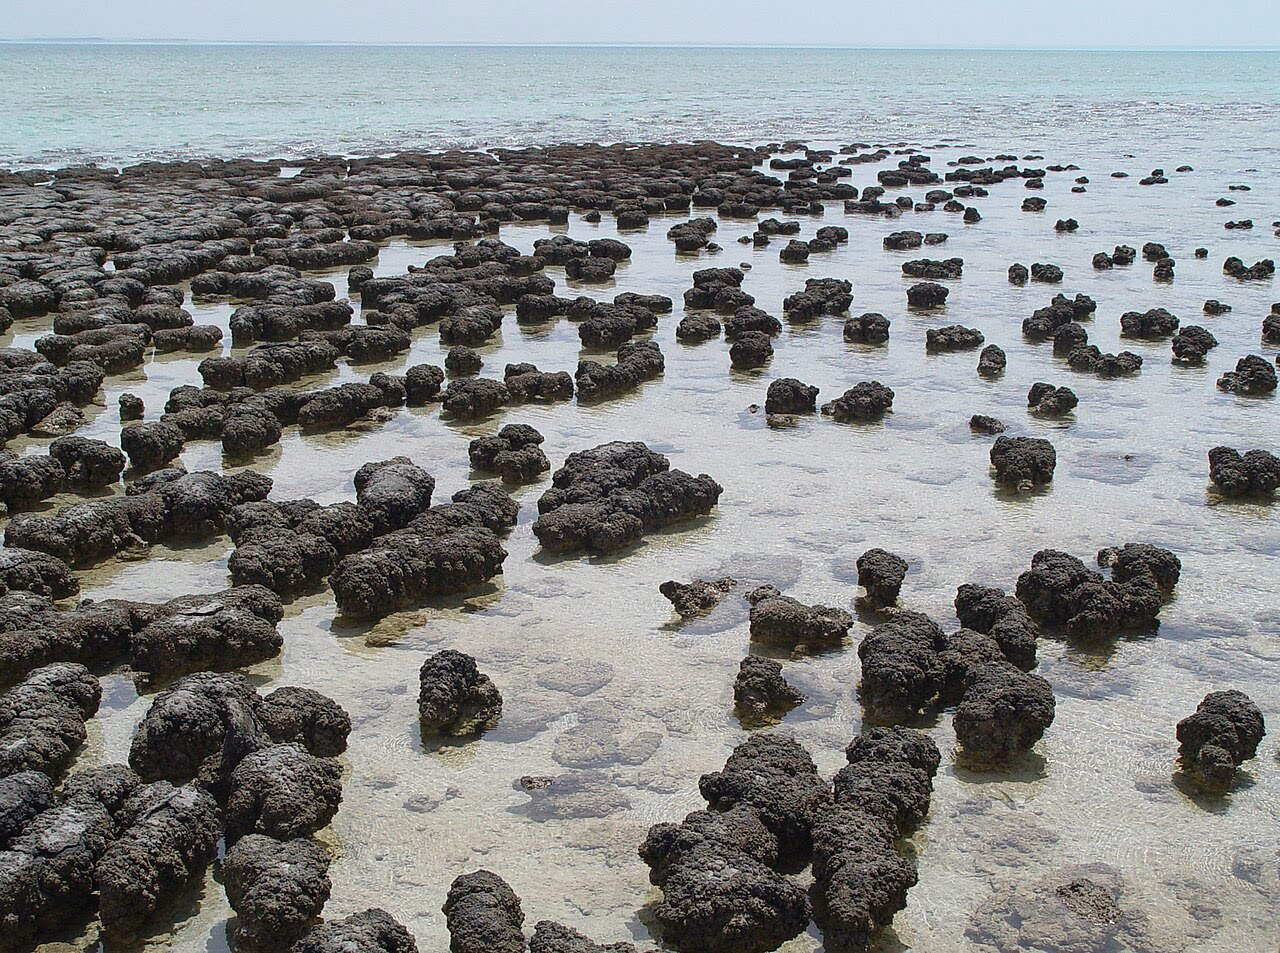
\includegraphics[width=0.6\linewidth]{images/book2/g12-shark-bay-stromatolites.jpg}

{\small \omterm{def:g12:early-earth:stromatolite}{Stromatolithes} vivants à Hamelin Pool, Shark Bay, Australie-Occidentale.
Photographie Paul Harrison, CC~BY-SA~3.0 (Wikimedia Commons).}
\end{omfigure}
% ledger: photo:g12-shark-bay

Les cyanobactéries apportèrent une nouveauté~: une photosynthèse qui libère
de l'oxygène. Mais longtemps, l'oxygène qu'elles produisaient ne resta pas
dans l'air. Il était consommé aussi vite qu'il était produit~: par le fer
dissous dans la mer, par le soufre et par le méthane.

\section{La montée de l'oxygène}

Avant l'oxygène, le fer pouvait voyager dissous dans l'eau de mer sous la
forme de l'ion \ce{Fe^2+}. L'oxygène le transforme en fer(III), qui ne se
dissout pas~: il tombe sur le fond en un sédiment couleur de rouille.

\begin{proposition}[Le fer fixe l'oxygène]\label{prop:g12:early-earth:iron}
Le fer(II) dissous est oxydé par l'oxygène, dans l'eau, en hydroxyde de
fer(III), qui précipite~:
\[
  \ce{4Fe^2+ + O2 + 10H2O -> 4Fe(OH)3 + 8H+} .
\]
Chaque molécule d'oxygène enlève quatre ions de fer dissous~; tant qu'il
reste du fer dissous, l'oxygène produit est consommé.
\end{proposition}
% ledger: earle:bif (ferrous iron oxidised to insoluble ferric iron)

\begin{proof}
Vérifions l'équilibre. Fer~: 4 de chaque côté. Oxygène~: $2 + 10 = 12$ à
gauche, $4 \times 3 = 12$ à droite. Hydrogène~: $20$ à gauche, $4 \times 3 + 8 =
20$ à droite. Charge~: $4 \times (+2) = +8$ à gauche, $8 \times (+1) =
+8$ à droite.
\end{proof}

\begin{definition}[Formation de fer rubané]\label{def:g12:early-earth:bif}
Une \emph{formation de fer rubané}\index{formation de fer rubane@formation de fer rubané}
est une roche sédimentaire faite de minces couches alternées d'oxydes de
fer, comme l'hématite, et de chert, une silice à grain fin pauvre en fer.
Presque toutes ont plus de 1.8~milliard d'années.
\end{definition}
% ledger: earle:bif, holland06:stages

Les \omterm{def:g12:early-earth:bif}{formations de fer rubané} exigent deux eaux à la fois~: un \omterm{def:g10:layered-ocean:thermocline}{océan
profond} sans oxygène, qui transporte du fer dissous, et une mer peu
profonde et ensoleillée où les cyanobactéries produisent de l'oxygène et où
le fer précipite. Elles sont fréquentes dans les roches âgées de 2.4 à
1.8~milliard d'années, et celles des monts Hamersley sont plus anciennes
encore. Les \omterm{def:g12:early-earth:bif}{formations de fer rubané} sont un minerai de fer courant.
% ledger: earle:bif, holland06:stages (Archean BIF, Hamersley), dbca:karijini

\begin{omfigure}
\begin{tikzpicture}[x=1cm, y=1cm, font=\scriptsize]
  % sea and floor
  \fill[omSea] (0,0) rectangle (11,4);
  \fill[omSea!45!white] (0,2.9) rectangle (11,4);
  \draw[omDef!60, line width=0.4pt, densely dashed] (0,2.9) -- (11,2.9);
  \node[anchor=north east, text=omDef] at (10.9,3.95) {eau de surface ensoleillée};
  \node[anchor=south east, text=omDef, align=right] at (10.9,0.12) {eau profonde\\sans oxygène,\\riche en \ce{Fe^2+}};
  % floor with layers
  \foreach \i/\c in {0/red!55!black, 1/black!20, 2/red!55!black, 3/black!20, 4/red!55!black, 5/black!20} {
    \fill[\c] (0,-0.12*\i) rectangle (11,-0.12*\i-0.12);
  }
  \draw[black!60] (0,0) -- (11,0);
  \node[anchor=west] at (11.1,-0.12) {oxyde de fer};
  \node[anchor=west] at (11.1,-0.36) {chert};
  \draw[black!50, line width=0.3pt] (11.05,-0.06) -- (10.6,-0.06);
  \draw[black!50, line width=0.3pt] (11.05,-0.30) -- (10.6,-0.30);
  % upwelling iron
  \foreach \x in {0.5,1.0,1.5} {
    \draw[-{Stealth}, omDef, line width=0.8pt] (\x,0.4) .. controls (\x+0.4,1.5) and (\x+0.6,2.2) .. (\x+0.9,2.85);
  }
  \node[text=omDef, anchor=west] at (2.3,1.3) {\ce{Fe^2+} remonte};
  % cyanobacteria and oxygen
  \foreach \x in {3.8,4.4,5.0,5.6,6.2} {\fill[green!45!black] (\x,3.35) circle (0.07);}
  \node[anchor=south, text=green!35!black] at (5.0,3.47) {les cyanobactéries produisent \ce{O2}};
  % reaction
  \node[draw=black!40, fill=white, rounded corners=2pt, inner sep=2pt] at (5.4,2.45) {\ce{4Fe^2+ + O2 + 10H2O -> 4Fe(OH)3 + 8H+}};
  % falling rust
  \foreach \x/\y in {4.6/1.9, 5.0/1.5, 5.5/1.8, 5.9/1.2, 4.3/1.1, 5.2/0.7, 6.1/0.6} {\fill[red!60!black] (\x,\y) circle (0.06);}
  \draw[-{Stealth}, red!60!black, line width=0.6pt] (6.6,2.1) -- (6.6,0.25);
  \node[anchor=west, text=red!60!black, align=left] at (6.7,1.75) {le fer(III) se dépose\\en une couche de rouille};
\end{tikzpicture}

{\small Comment se forme une \omterm{def:g12:early-earth:bif}{formation de fer rubané} (schéma, sans
échelle)~: le fer dissous dans l'eau profonde, qui ne contient pas
d'oxygène, remonte dans la mer ensoleillée, où l'oxygène produit par les
cyanobactéries le transforme en fer(III), qui se dépose. Des couches riches
en fer alternent avec des couches de chert.}
\end{omfigure}

Puis l'oxygène commença à rester dans l'air.

\begin{definition}[Grande Oxydation]\label{def:g12:early-earth:goe}
La \emph{Grande Oxydation}\index{Grande Oxydation} est l'intervalle, d'il y
a environ \num{2.46} à environ \num{2.06}~milliards d'années, pendant
lequel l'oxygène libre s'est accumulé pour la première fois dans
l'atmosphère et les mers peu profondes de la Terre, atteignant peut-être le
dixième de sa teneur actuelle.
\end{definition}
% ledger: gumsley17:goe, holland06:stages (0.02-0.04 atm, about a tenth of 0.21)

Les preuves sont dans les roches. Certains minéraux, dont la pyrite et
l'uraninite, sont détruits par l'oxygène~; pourtant, on en trouve des
grains, roulés par les rivières, dans des sédiments anciens, et les grains
de pyrite manquent dans ceux qui se sont déposés après la montée de
l'oxygène. Les isotopes du soufre des roches de plus de 2.45~milliards
d'années environ portent une signature que seul un air contenant moins
d'un cent-millième de l'oxygène actuel peut laisser~; il y a 2.09~milliards
d'années, elle a disparu. Et sur les continents apparurent les \omterm{def:g12:early-earth:red-beds}{couches
rouges}.
% ledger: kasting25:indicators, pk02:anoxic, farquhar00:sulfur

\begin{definition}[Couches rouges]\label{def:g12:early-earth:red-beds}
Les \emph{couches rouges}\index{couches rouges} sont des roches
sédimentaires --- grès, siltites, argilites --- colorées en rouge par un
enduit d'oxyde de fer(III), l'hématite, sur leurs grains. Elles ne se
forment que là où il y a assez d'oxygène pour oxyder le fer.
\end{definition}
% ledger: kasting25:indicators (redbeds an oxygen indicator)

\begin{omfigure}
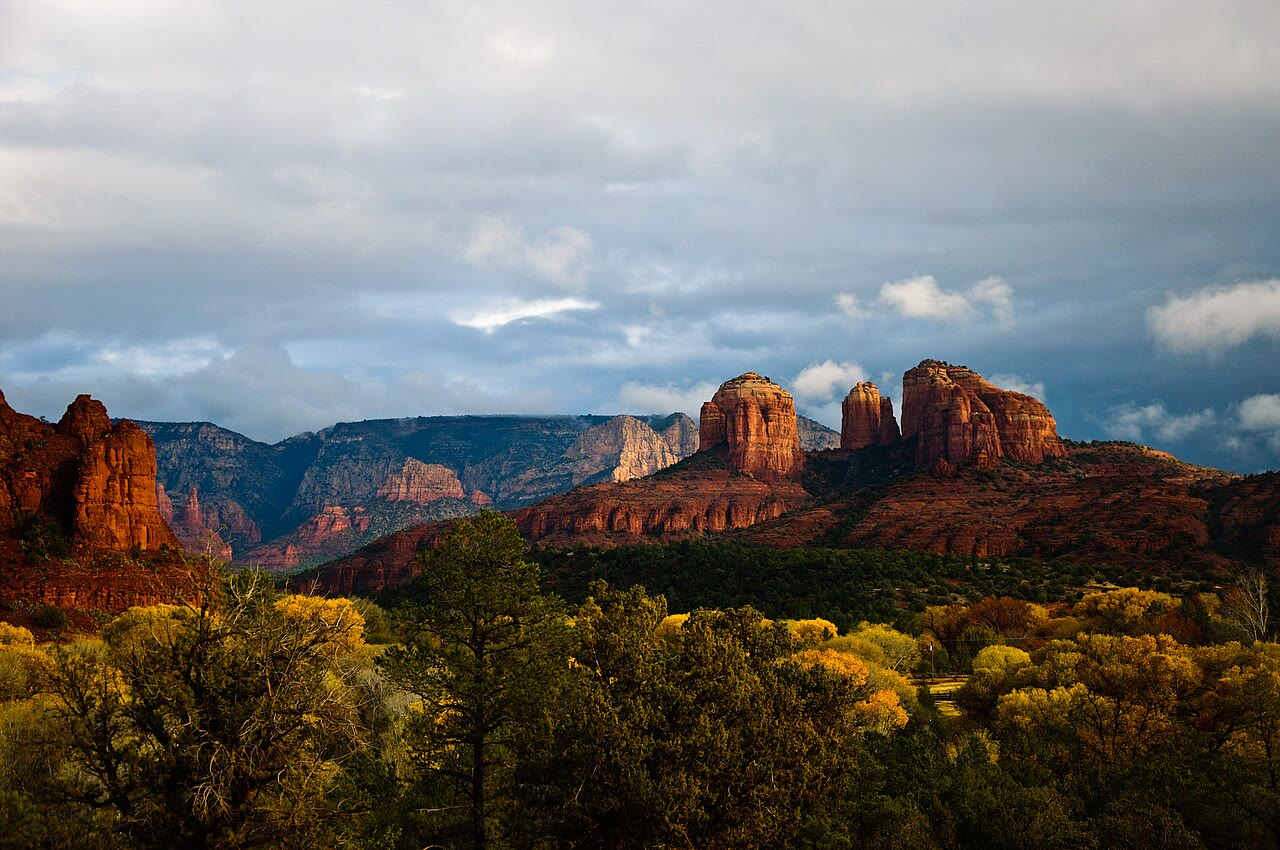
\includegraphics[width=0.66\linewidth]{images/book2/g12-sedona-red-beds.jpg}

{\small Des \omterm{def:g12:early-earth:red-beds}{couches rouges}~: Cathedral Rock, près de Sedona, en Arizona,
faite de grès rouges du Permien. Photographie Wendy from Pennsylvania,
CC~BY-SA~2.0 (Wikimedia Commons).}
\end{omfigure}
% ledger: photo:g12-sedona, azgs:cathedral (Permian Schnebly Hill Sandstone)

Le dépôt des \omterm{def:g12:early-earth:bif}{formations de fer rubané} a pour l'essentiel cessé après
1.8~milliard d'années avant l'actuel~: l'\omterm{def:g10:layered-ocean:thermocline}{océan profond} contenait alors lui
aussi assez d'oxygène pour ne plus transporter de fer. Pendant le milliard
d'années suivant, l'oxygène changea peu~; après 0.85~milliard d'années
avant l'actuel, il augmenta de nouveau, vers les \qty{21}{\percent}
actuels.
% ledger: earle:bif, holland06:stages

\begin{method}[Lire une frise chronologique géologique]\label{met:g12:early-earth:timeline}
\begin{enumerate}
  \item Repérer dans quel sens le temps s'écoule sur l'axe, et son unité
        (millions ou milliards d'années avant l'actuel).
  \item Situer les éons sur la bande colorée, et lire leurs limites.
  \item Pour chaque événement, lire sa date, ou l'intervalle pendant lequel
        il s'est produit, et dire quel enregistrement le date (un minéral,
        un fossile, une roche).
  \item Calculer les durées par soustraction, et les comparer à l'\omterm{def:g12:age-of-the-earth:age}{âge de la
        Terre}.
  \item Vérifier l'ordre~: un effet ne doit pas précéder sa cause.
\end{enumerate}
\end{method}

\begin{omfigure}
\begin{tikzpicture}
\begin{axis}[omrecord, width=0.82\linewidth, height=6.2cm, ymode=log, xmin=0, xmax=4.6, ymin=1e-7, ymax=5,
  x dir=reverse, xlabel={temps avant l'actuel (milliards d'années)}, ylabel={oxygène dans l'air (actuel $=1$)},
  xtick={0,0.5,...,4.5}, x tick label style={/pgf/number format/.cd, fixed, precision=1},
  ytick={1e-6,1e-4,1e-2,1}, ymajorgrids=true, xmajorgrids=false, clip=false]
% computed in figdata/grade-12/early_earth.py (schematic through the sourced bounds); ledger: holland06:stages, pk02:anoxic, gumsley17:goe, ics:base.Hadean, ics:base.Archean, ics:base.Proterozoic, ics:base.Paleozoic
\fill[omThm!12] (axis cs:2.46,1e-7) rectangle (axis cs:2.06,5);
\addplot[black, line width=1.2pt] table[x=t_Ga, y=pal] {figdata/out/grade-12-early_earth-oxygen.dat};
% eon band (ICS colours), below the axis
\fill[icsHadean] (axis cs:4.567,1.5e-7) rectangle (axis cs:4.031,4e-7);
\fill[icsArchean] (axis cs:4.031,1.5e-7) rectangle (axis cs:2.5,4e-7);
\fill[icsProterozoic] (axis cs:2.5,1.5e-7) rectangle (axis cs:0.5388,4e-7);
\fill[icsPhanerozoic] (axis cs:0.5388,1.5e-7) rectangle (axis cs:0,4e-7);
\node[font=\tiny, text=white] at (axis cs:4.30,2.45e-7) {Hadéen};
\node[font=\tiny, text=white] at (axis cs:3.27,2.45e-7) {Archéen};
\node[font=\tiny, text=white] at (axis cs:1.52,2.45e-7) {Protérozoïque};
% events
\draw[omDef, line width=0.6pt] (axis cs:4.4,4e-7) -- (axis cs:4.4,3e-3);
\node[font=\scriptsize, text=omDef, anchor=south west] at (axis cs:4.4,3e-3) {zircons, eau};
\draw[omMeth, line width=0.6pt] (axis cs:3.43,4e-7) -- (axis cs:3.43,1.2e-6);
\node[font=\scriptsize, text=omMeth, anchor=south] at (axis cs:3.43,1.2e-6) {premiers stromatolithes};
\draw[red!60!black, line width=3pt] (axis cs:2.4,3e-6) -- (axis cs:1.8,3e-6);
\node[font=\scriptsize, text=red!60!black, anchor=north] at (axis cs:2.16,2.4e-6) {formations de fer rubané};
\node[font=\scriptsize, text=omThm, anchor=south, align=center] at (axis cs:2.26,1.2) {Grande\\Oxydation};
\node[font=\scriptsize, anchor=south] at (axis cs:3.2,1.3e-5) {moins de $10^{-5}$ de l'actuel};
\node[font=\scriptsize, anchor=south] at (axis cs:1.4,0.12) {environ un dixième};
\end{axis}
\end{tikzpicture}

{\small L'oxygène dans l'air au cours du temps (schéma, échelle
logarithmique)~: la courbe relie les bornes mesurées et masque les hauts et
les bas de l'enregistrement réel. L'intervalle grisé est la \omterm{def:g12:early-earth:goe}{Grande
Oxydation}~; la barre rouge marque l'époque où les \omterm{def:g12:early-earth:bif}{formations de fer rubané}
étaient fréquentes, il y a 2.4 à 1.8~milliard d'années. Éons d'après la
Charte chronostratigraphique internationale.}
\end{omfigure}

\section{Exercices}

\begin{exercise}[$\star$]\label{exo:g12:early-earth:1}
Donner le mot~: (a) la libération des gaz dissous dans le magma~; (b) un
monticule lité construit par un tapis microbien~; (c) une roche faite de
couches alternées d'oxyde de fer et de chert~; (d) des roches
sédimentaires colorées par l'hématite~; (e) l'intervalle pendant lequel
l'oxygène s'est accumulé pour la première fois dans l'air.
\end{exercise}

\begin{exercise}[$\star$]\label{exo:g12:early-earth:2}
Ranger dans l'ordre, du plus ancien au plus récent~: la fin de la plupart
des \omterm{def:g12:early-earth:bif}{formations de fer rubané}~; les premiers \omterm{def:g12:early-earth:stromatolite}{stromatolithes} du Pilbara~; les
zircons qui montrent de l'eau liquide~; les \omterm{def:g12:early-earth:bif}{formations de fer rubané} des
monts Hamersley~; la fin de la \omterm{def:g12:early-earth:goe}{Grande Oxydation}.
\end{exercise}

\begin{exercise}[$\star$]\label{exo:g12:early-earth:3}
À l'aide de la loi de luminosité, calculer la luminosité du Soleil à sa
naissance, en fraction de la luminosité actuelle. De quel pourcentage
était-il moins lumineux~?
\end{exercise}

\begin{exercise}[$\star$]\label{exo:g12:early-earth:4}
On trouve des grains de pyrite roulés par les rivières dans des sédiments
anciens, mais pas dans ceux qui se sont déposés après la montée de
l'oxygène. Qu'est-ce que cela apprend sur l'air à l'époque des sédiments
anciens~? Pourquoi~?
\end{exercise}

\begin{exercise}[$\star$]\label{exo:g12:early-earth:5}
Nommer les deux gaz les plus abondants libérés par les volcans, et dire ce
que chacun est devenu sur la jeune Terre.
\end{exercise}

\begin{exercise}[$\star\star$]\label{exo:g12:early-earth:6}
Calculer la luminosité du Soleil et la \omterm{def:g10:habitable-planet:equilibrium-temperature}{température d'équilibre} de la Terre
(aujourd'hui \qty{255}{K}, \omterm{def:g10:earth-energy-budget:albedo}{albédo} inchangé) il y a 3~milliards d'années et
il y a 2.45~milliards d'années, en prenant $t_\odot = 4.567$~milliards
d'années.
\end{exercise}

\begin{exercise}[$\star\star$]\label{exo:g12:early-earth:7}
Quelle masse d'oxygène faut-il pour précipiter \qty{1}{kg} de fer dissous
sous forme d'hydroxyde de fer(III)~? (Masses molaires~: fer
\qty{55.85}{g/mol}, oxygène \qty{16.00}{g/mol}.)
\end{exercise}

\begin{exercise}[$\star\star$]\label{exo:g12:early-earth:8}
À l'aide de la frise chronologique, (1) combien de temps la \omterm{def:g12:early-earth:goe}{Grande
Oxydation} a-t-elle duré~? (2) Pendant quelle fraction de l'histoire de la
Terre n'y a-t-il eu presque pas d'oxygène dans l'air~? (3) Combien de temps
après les premiers \omterm{def:g12:early-earth:stromatolite}{stromatolithes} l'oxygène a-t-il commencé à s'accumuler~?
\end{exercise}

\begin{exercise}[$\star\star$]\label{exo:g12:early-earth:9}
Une \omterm{def:g12:early-earth:bif}{formation de fer rubané} et une couche rouge contiennent toutes deux de
l'oxyde de fer(III). Qu'apprend chacune sur l'oxygène, et où~: dans la mer
profonde, dans la mer peu profonde, dans l'air~?
\end{exercise}

\begin{exercise}[$\star\star$]\label{exo:g12:early-earth:10}
Où peut-on voir aujourd'hui des \omterm{def:g12:early-earth:stromatolite}{stromatolithes} vivants~? Qu'a de
particulier l'eau à cet endroit, et comment un \omterm{def:g12:early-earth:stromatolite}{stromatolithe} croît-il
couche après couche~?
\end{exercise}

\begin{exercise}[$\star\star$]\label{exo:g12:early-earth:11}
L'oxygène représente \qty{21}{\percent} de l'air actuel. Quel pourcentage
représentait-il quand il était (1) au cent-millième de sa teneur
actuelle~; (2) au dixième de sa teneur actuelle~?
\end{exercise}

\begin{exercise}[$\star\star\star$]\label{exo:g12:early-earth:12}
Il y a quatre milliards d'années, quel \omterm{def:g10:earth-energy-budget:albedo}{albédo} aurait donné à la Terre la
\omterm{def:g10:habitable-planet:equilibrium-temperature}{température d'équilibre} actuelle, \qty{255}{K}, sous le jeune Soleil
($L = 0.741\,L_\odot$, \omterm{def:g10:earth-energy-budget:albedo}{albédo} actuel 0.294)~? Une planète dotée d'un océan,
de nuages et d'un peu de glace a-t-elle des chances d'avoir été aussi
sombre~? Quelle est l'autre issue~?
\end{exercise}

\begin{exercise}[$\star\star\star$]\label{exo:g12:early-earth:13}
Aujourd'hui, l'effet de serre réchauffe la surface de la Terre de 255 à
\qty{288}{K}. Il y a quatre milliards d'années, la \omterm{def:g10:habitable-planet:equilibrium-temperature}{température d'équilibre}
était d'environ \qty{237}{K}. (1) Combien de kelvins de réchauffement par
effet de serre fallait-il alors pour atteindre \qty{273}{K}~? Pour
atteindre \qty{288}{K}~? (2) Comparer à la valeur actuelle. (3) Un calcul
classique demande environ \qty{0.1}{bar} de dioxyde de carbone, avec un peu
de méthane~; comparer à la pression de toute l'atmosphère actuelle,
environ \qty{1}{bar}.
\end{exercise}

\begin{exercise}[$\star\star\star$]\label{exo:g12:early-earth:14}
Une signature particulière des isotopes du soufre ne peut être produite, et
conservée dans les sédiments, que si l'air contient moins de $10^{-5}$ de
l'oxygène actuel. On la trouve dans des roches de plus de 2450 millions
d'années, et pas dans des roches de moins de 2090 millions d'années.
(1) Que conclure sur l'oxygène avant 2450 millions d'années~? Après 2090
millions d'années~? (2) Est-ce cohérent avec les dates de la \omterm{def:g12:early-earth:goe}{Grande
Oxydation}~?
\end{exercise}

\begin{exercise}[$\star\star\star$]\label{exo:g12:early-earth:15}
L'impact qui a formé la Lune s'est produit environ 60 millions d'années
après le début de la formation du système solaire, que les premiers
solides datent d'il y a 4567 millions d'années. (1) À quelle date environ
l'impact s'est-il produit~? (2) Les plus vieux zircons ont \num{4404}
millions d'années. Au plus combien de temps après l'impact la Terre
avait-elle déjà une croûte solide et de l'eau liquide~?
\end{exercise}
% ledger: nasa:moon-formation, connelly12:cai, wilde01:4404

\begin{problem}[{Problème du week-end --- le jeune Soleil faible}]
\label{pb:g12:early-earth:1}
% ledger: gough81:luminosity, connelly12:cai, earth:TSI, earth:albedo, earth:Tsurf, feulner12:fys, allwood06:spc, dbca:karijini, wilde01:zircon
% values (early_earth.py): L_4Ga 0.7406, S_4Ga 1007.9, Teq_today 255.1, Teq_4Ga 236.7, albedo_needed 0.047
Le Soleil a \num{4.567}~milliards d'années. Sa luminosité quand il avait
$t$ années valait $L(t) = L_\odot/\bigl(1 + \tfrac25 (1 - t/t_\odot)\bigr)$.
Aujourd'hui, la Terre reçoit \qty{1361}{W/m^2} de lumière solaire, en
réfléchit une fraction 0.294, et a une \omterm{def:g10:habitable-planet:equilibrium-temperature}{température d'équilibre} de
\qty{255}{K}~; sa température moyenne de surface est de \qty{288}{K}.

\medskip
\noindent\textbf{Partie I --- Le Soleil il y a quatre milliards d'années.}
\begin{enumerate}
  \item Quel âge avait le Soleil il y a quatre milliards d'années~?
  \item Calculer $1 - t/t_\odot$ à cette époque.
  \item Calculer sa luminosité en fraction de la luminosité actuelle.
  \item Quelle lumière solaire la Terre recevait-elle, en \unit{W/m^2}~?
  \item De quel pourcentage le Soleil était-il moins lumineux
        qu'aujourd'hui~?
\end{enumerate}

\medskip
\noindent\textbf{Partie II --- La température d'équilibre.}
\begin{enumerate}[resume]
  \item Écrire la \omterm{def:g10:habitable-planet:equilibrium-temperature}{température d'équilibre} en fonction de la lumière
        solaire $S$.
  \item Montrer que, à \omterm{def:g10:earth-energy-budget:albedo}{albédo} inchangé, la température varie comme
        $S^{1/4}$.
  \item Calculer $0.741^{1/4}$.
  \item Calculer la \omterm{def:g10:habitable-planet:equilibrium-temperature}{température d'équilibre} il y a quatre milliards
        d'années.
  \item La convertir en degrés Celsius.
\end{enumerate}

\medskip
\noindent\textbf{Partie III --- Les preuves de l'eau liquide.}
\begin{enumerate}[resume]
  \item Que montrent les zircons de 4.4~milliards d'années~?
  \item Dans quel type d'eau les \omterm{def:g12:early-earth:stromatolite}{stromatolithes} du Pilbara, âgés de
        \num{3430} millions d'années, ont-ils poussé~?
  \item Quelles roches des monts Hamersley, déposées dans la mer il y a
        plus de 2.5~milliards d'années, exigent de l'eau liquide~?
  \item Sans effet de serre, l'océan aurait-il gelé il y a quatre milliards
        d'années~? Pourquoi~?
  \item Énoncer la contradiction que cela révèle, et donner son nom.
\end{enumerate}

\medskip
\noindent\textbf{Partie IV --- Le réchauffement par effet de serre nécessaire.}
\begin{enumerate}[resume]
  \item Combien de kelvins l'effet de serre actuel ajoute-t-il~?
  \item Combien en fallait-il il y a quatre milliards d'années pour
        maintenir la surface moyenne au-dessus de \qty{273}{K}~?
  \item Quel \omterm{def:g10:earth-energy-budget:albedo}{albédo} aurait donné \qty{255}{K} sans aucun effet de serre
        supplémentaire~? Est-ce plausible~?
  \item Quel gaz aurait fourni l'essentiel du réchauffement
        supplémentaire, et quel autre gaz a pu y contribuer~?
  \item Résumer~: quelle était la \omterm{def:g10:habitable-planet:equilibrium-temperature}{température d'équilibre} de la Terre il y
        a quatre milliards d'années~?
\end{enumerate}
\end{problem}
